\documentclass[border=10pt]{standalone}
\usepackage{tikz}
\usetikzlibrary{shapes.geometric, arrows.meta, positioning, calc, fit, backgrounds, shadows.blur, decorations.pathmorphing}
\usepackage[T1]{fontenc}
\usepackage{helvet}
\renewcommand{\familydefault}{\sfdefault}

\definecolor{morphorange}{HTML}{FF6B2B}
\definecolor{morphdark}{HTML}{0D0D1A}
\definecolor{morphgray}{HTML}{1A1A2E}
\definecolor{morphblue}{HTML}{4A90D9}
\definecolor{morphpurple}{HTML}{8B5CF6}
\definecolor{morphgreen}{HTML}{10B981}
\definecolor{morphaccent}{HTML}{F59E0B}
\definecolor{textwhite}{HTML}{F0F0F0}
\definecolor{textgray}{HTML}{9CA3AF}
\definecolor{cardbg}{HTML}{16162A}

\begin{document}
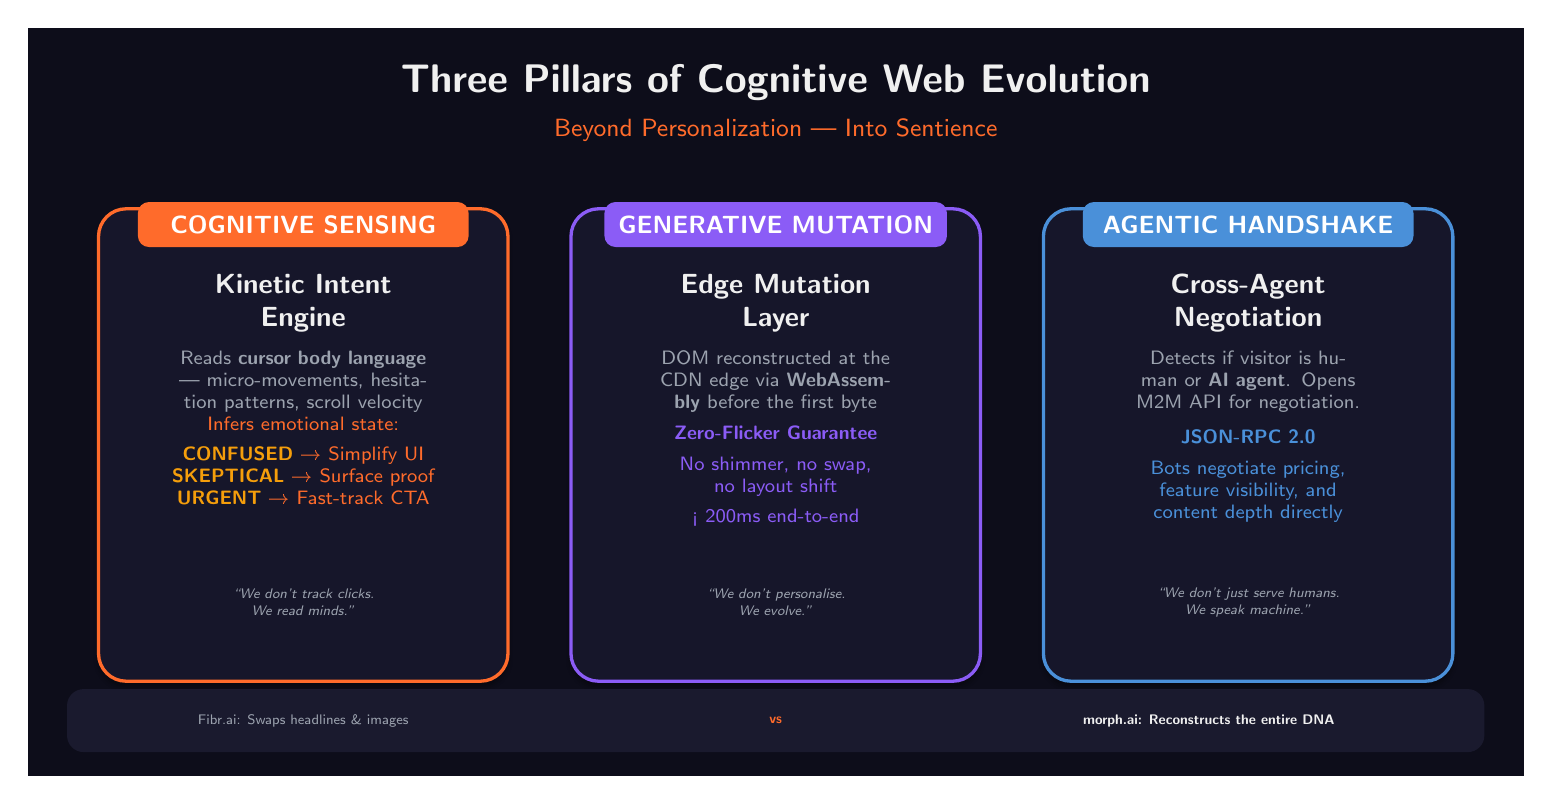
\begin{tikzpicture}[
    every node/.style={font=\sffamily},
]

% Background
\fill[morphdark] (-9.5,-5) rectangle (9.5,4.5);

% Title
\node[text=textwhite, font=\sffamily\bfseries\Large] at (0,3.8) {Three Pillars of Cognitive Web Evolution};
\node[text=morphorange, font=\sffamily\small] at (0,3.2) {Beyond Personalization — Into Sentience};

% === PILLAR 1: Cognitive Sensing ===
\node[draw=morphorange, fill=cardbg, rounded corners=10pt, minimum width=5.2cm, minimum height=6cm,
      line width=1.2pt, blur shadow={shadow blur steps=5, shadow xshift=0pt, shadow yshift=-2pt}] 
      (p1) at (-6, -0.8) {};

\node[fill=morphorange, rounded corners=4pt, text=white, font=\sffamily\bfseries\small, inner sep=5pt, minimum width=4.2cm] 
      at (-6, 2) {COGNITIVE SENSING};

\node[text=textwhite, font=\sffamily\bfseries, text width=4.5cm, align=center] at (-6, 1.0) 
      {Kinetic Intent\\Engine};

\node[text=textgray, font=\sffamily\scriptsize, text width=4.2cm, align=center] at (-6, 0.0) 
      {Reads \textbf{cursor body language} — micro-movements, hesitation patterns, scroll velocity};

\node[text=morphorange, font=\sffamily\scriptsize, text width=4.2cm, align=center] at (-6, -1.0) 
      {Infers emotional state:\\[3pt]
      \textcolor{morphaccent}{\textbf{CONFUSED}} → Simplify UI\\
      \textcolor{morphaccent}{\textbf{SKEPTICAL}} → Surface proof\\
      \textcolor{morphaccent}{\textbf{URGENT}} → Fast-track CTA};

\node[text=textgray, font=\sffamily\tiny\itshape, text width=4cm, align=center] at (-6, -2.8) 
      {``We don't track clicks.\\We read minds.''};

% === PILLAR 2: Generative Mutation ===
\node[draw=morphpurple, fill=cardbg, rounded corners=10pt, minimum width=5.2cm, minimum height=6cm,
      line width=1.2pt, blur shadow={shadow blur steps=5, shadow xshift=0pt, shadow yshift=-2pt}] 
      (p2) at (0, -0.8) {};

\node[fill=morphpurple, rounded corners=4pt, text=white, font=\sffamily\bfseries\small, inner sep=5pt, minimum width=4.2cm] 
      at (0, 2) {GENERATIVE MUTATION};

\node[text=textwhite, font=\sffamily\bfseries, text width=4.5cm, align=center] at (0, 1.0) 
      {Edge Mutation\\Layer};

\node[text=textgray, font=\sffamily\scriptsize, text width=4.2cm, align=center] at (0, 0.0) 
      {DOM reconstructed at the CDN edge via \textbf{WebAssembly} before the first byte};

\node[text=morphpurple, font=\sffamily\scriptsize, text width=4.2cm, align=center] at (0, -1.2) 
      {\textbf{Zero-Flicker Guarantee}\\[3pt]
      No shimmer, no swap,\\no layout shift\\[3pt]
      < 200ms end-to-end};

\node[text=textgray, font=\sffamily\tiny\itshape, text width=4cm, align=center] at (0, -2.8) 
      {``We don't personalise.\\We evolve.''};

% === PILLAR 3: Agentic Handshake ===
\node[draw=morphblue, fill=cardbg, rounded corners=10pt, minimum width=5.2cm, minimum height=6cm,
      line width=1.2pt, blur shadow={shadow blur steps=5, shadow xshift=0pt, shadow yshift=-2pt}] 
      (p3) at (6, -0.8) {};

\node[fill=morphblue, rounded corners=4pt, text=white, font=\sffamily\bfseries\small, inner sep=5pt, minimum width=4.2cm] 
      at (6, 2) {AGENTIC HANDSHAKE};

\node[text=textwhite, font=\sffamily\bfseries, text width=4.5cm, align=center] at (6, 1.0) 
      {Cross-Agent\\Negotiation};

\node[text=textgray, font=\sffamily\scriptsize, text width=4.2cm, align=center] at (6, 0.0) 
      {Detects if visitor is human or \textbf{AI agent}. Opens M2M API for negotiation.};

\node[text=morphblue, font=\sffamily\scriptsize, text width=4.2cm, align=center] at (6, -1.2) 
      {\textbf{JSON-RPC 2.0}\\[3pt]
      Bots negotiate pricing,\\feature visibility, and\\content depth directly};

\node[text=textgray, font=\sffamily\tiny\itshape, text width=4cm, align=center] at (6, -2.8) 
      {``We don't just serve humans.\\We speak machine.''};

% === Bottom comparison bar ===
\node[fill=morphgray, rounded corners=6pt, minimum width=18cm, minimum height=0.8cm, draw=none] at (0, -4.3) {};
\node[text=textgray, font=\sffamily\tiny] at (-6, -4.3) {Fibr.ai: Swaps headlines \& images};
\node[text=morphorange, font=\sffamily\tiny\bfseries] at (0, -4.3) {vs};
\node[text=textwhite, font=\sffamily\tiny\bfseries] at (5.5, -4.3) {morph.ai: Reconstructs the entire DNA};

\end{tikzpicture}
\end{document}
